
\documentclass[12pt,letterpaper]{article}

\usepackage[margin=1in]{geometry}
\usepackage{amsmath,amssymb}
\usepackage{booktabs}
\usepackage{graphicx}
\usepackage{hyperref}
\usepackage{enumitem}
\usepackage{caption}
\usepackage{array}
\usepackage{parskip}
\usepackage{float}
\usepackage{longtable}

\hypersetup{
    colorlinks=true,
    linkcolor=blue,
    urlcolor=blue
}

\begin{document}

\begin{titlepage}
\centering
\vspace*{1.2cm}

{\Large MIE312: Lab 4\par}
\vspace{0.5em}
{\Huge\bfseries Impulse Turbines: Application of Fluid Momentum Principles\par}
\vspace{1.2em}

{\Large Department of Mechanical and Industrial Engineering\par}
{\Large University of Toronto\par}
\textcolor{white}{\Large Prepared by: Prof. Sullivan} \\
{\Large Fall 2026}

\vfill

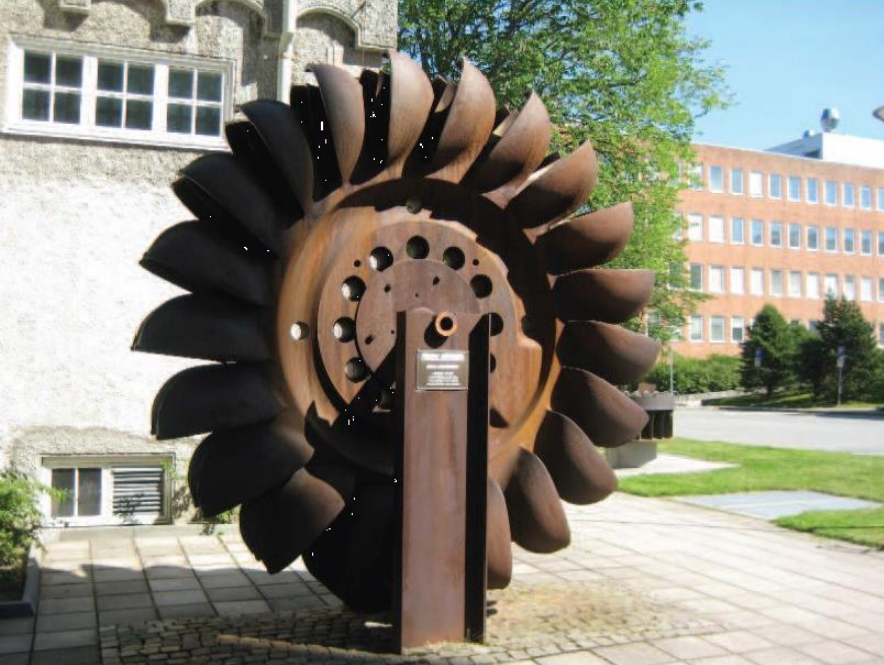
\includegraphics[width=0.58\textwidth]{Lab4_Figures/Lab4_cover.png}\par

\vfill

\begin{tabular}{|p{0.28\textwidth}|p{0.44\textwidth}|}
\hline
Teaching Assistant: & Hesam Banejad \\ \hline
Email: & \small\nolinkurl{a.banejad@mail.utoronto.ca} \\ \hline
\end{tabular}

\vfill
\end{titlepage}

\section*{Companion Notebook}

A Google Colab notebook accompanies this lab manual. It automates the calculation of jet velocity, shaft torque, brake power, water power, experimental efficiency, and theoretical efficiency, and generates the efficiency-versus-\(\phi\) plots for both turbine geometries after the raw measurements are entered.

\begin{center}
\href{https://colab.research.google.com/github/pierresullivan/mie312-labs/blob/main/lab4-turbines/MIE312_Lab4_Impulse_Turbines.ipynb}{\textbf{Open the MIE312 Lab 4 Colab Notebook}}
\end{center}

\subsection*{How students should use the notebook}
\begin{enumerate}[leftmargin=*, label=\arabic*.]
    \item Open the notebook and save a personal copy.
    \item Run the setup cells first so the constants, geometry, and helper functions are defined.
    \item Enter the raw measurements for pressure, flow rate, brake-load readings, and angular velocity for both turbines.
    \item Run the remaining cells to compute torque, angular speed, blade speed, jet speed, water power, brake power, and both theoretical and measured efficiencies.
    \item Copy the generated tables, plots, and discussion prompts into the final report as needed.
\end{enumerate}
\vspace{1em}
\hrule
\vspace{1em}

\section{Objective}
The objectives of this lab experiment are to:
\begin{itemize}[leftmargin=*]
    \item measure the efficiencies of two impulse turbines with different blade geometries,
    \item determine how turbine efficiency depends on blade shape,
    \item compare measured efficiencies with theoretical predictions,
    \item determine which blade design is more efficient.
\end{itemize}

\section{Experimental Setup}
The original lab manual describes a turbine station mounted on a hydraulic bench. Water is pumped through a hose to an impulse turbine, where the water jet strikes the runner blades and produces torque on the shaft. A brake drum and two load gauges are used to measure the resisting torque, and the rotational speed is measured using either a stroboscope or a tachometer.

\subsection*{Hydraulic-bench and turbine-station components}
The manual identifies the following main components of the hydraulic bench and turbine station:
\begin{enumerate}[leftmargin=*, label=\arabic*.]
    \item Hydraulic bench
    \item Power switch
    \item Flow valve
    \item Water hose
\end{enumerate}

For the turbine itself, the manual identifies:
\begin{enumerate}[leftmargin=*, label=\arabic*.]
    \item Load adjust controls
    \item Left and right load gauges
    \item Inlet pressure gauge
\end{enumerate}

Two turbines are used:
\begin{itemize}[leftmargin=*]
    \item a \textbf{flat-blade turbine} with blade deflection angle \(\beta = 90^\circ\),
    \item a \textbf{Pelton-type bucket turbine} with blade angle \(\beta = 160^\circ\).
\end{itemize}

The brake pulley is located at the back of each turbine. Two different radii are required in the data reduction and must not be confused:
\[
R_d = 25~\text{mm} = 0.025~\text{m}
\]
is the \textbf{brake-drum radius} used only to convert the measured brake force to shaft torque, while
\[
r_b = 46~\text{mm} = 0.046~\text{m}
\]
is the \textbf{effective turbine (blade) radius} used to calculate the blade peripheral speed and the angular-momentum model. The value \(r_b=46~\text{mm}\) is the manufacturer value for the TecQuipment H19 Pelton turbine geometry. The flat-blade runner used in this lab is otherwise geometrically identical to the Pelton unit; if the installed hardware differs, use the value confirmed by the TA.

\begin{figure}[H]
    \centering
    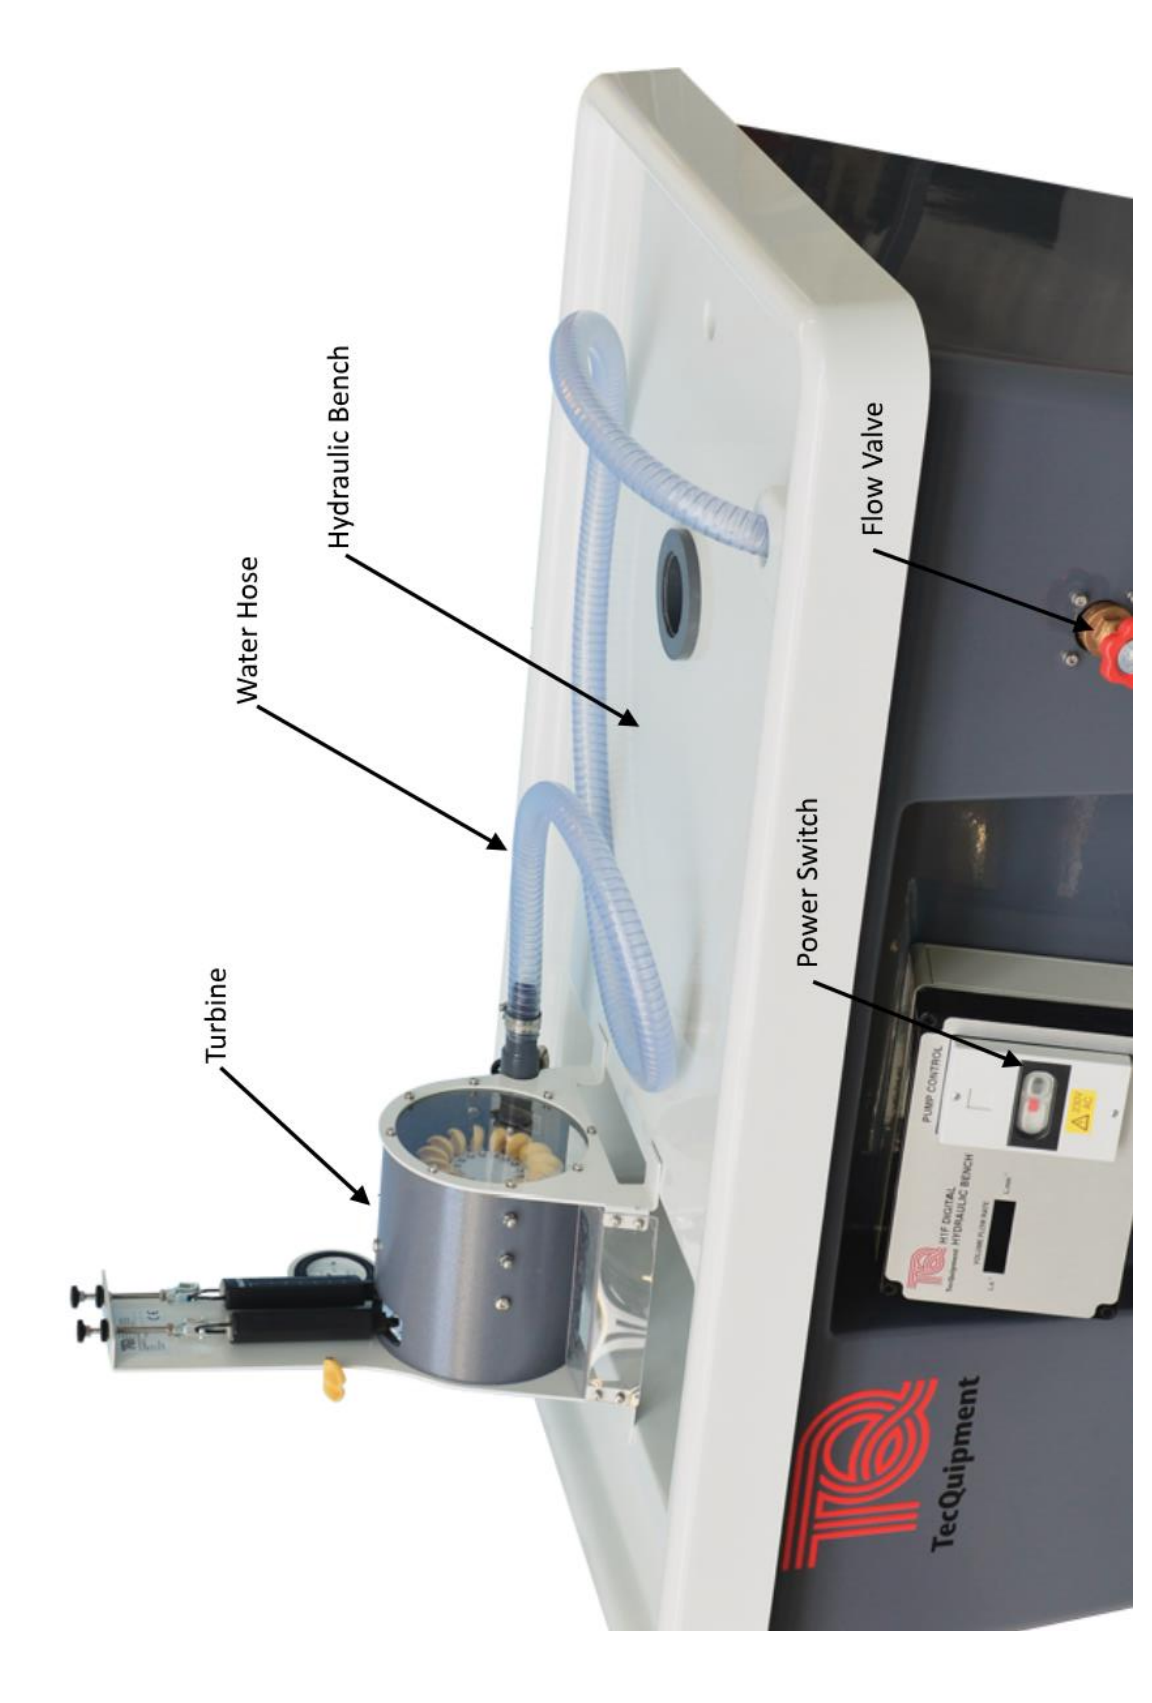
\includegraphics[angle=270,width=0.68\textheight]{Lab4_Figures/apparatus_overview.png}
    \caption{Hydraulic bench and turbine apparatus overview.}
    \label{fig:apparatus-overview}
\end{figure}

\begin{figure}[H]
    \centering
    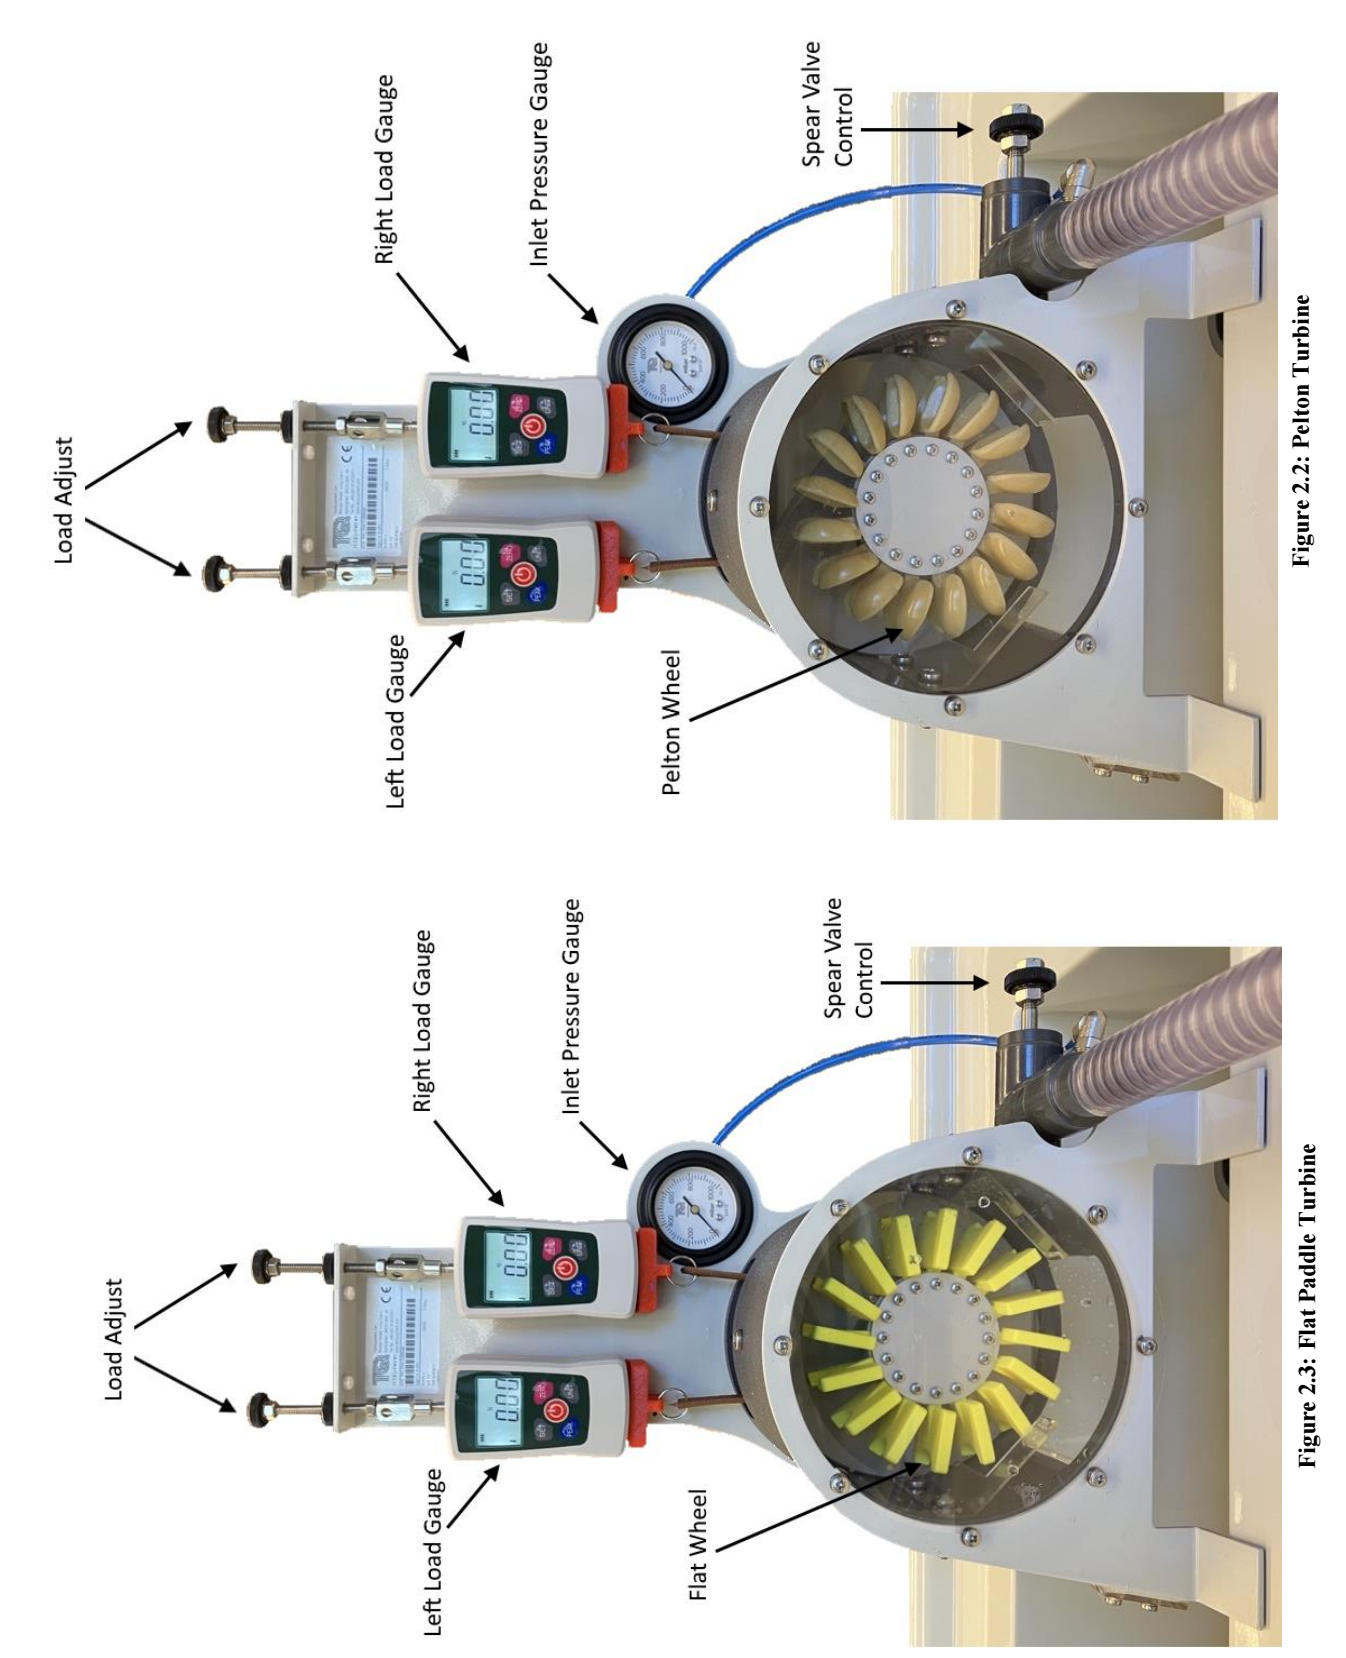
\includegraphics[angle=270,width=0.68\textheight]{Lab4_Figures/turbine_types.png}
    \caption{Impulse turbine blade geometries used in the experiment: flat blade and Pelton bucket.}
    \label{fig:turbine-types}
\end{figure}

\begin{figure}[H]
    \centering
    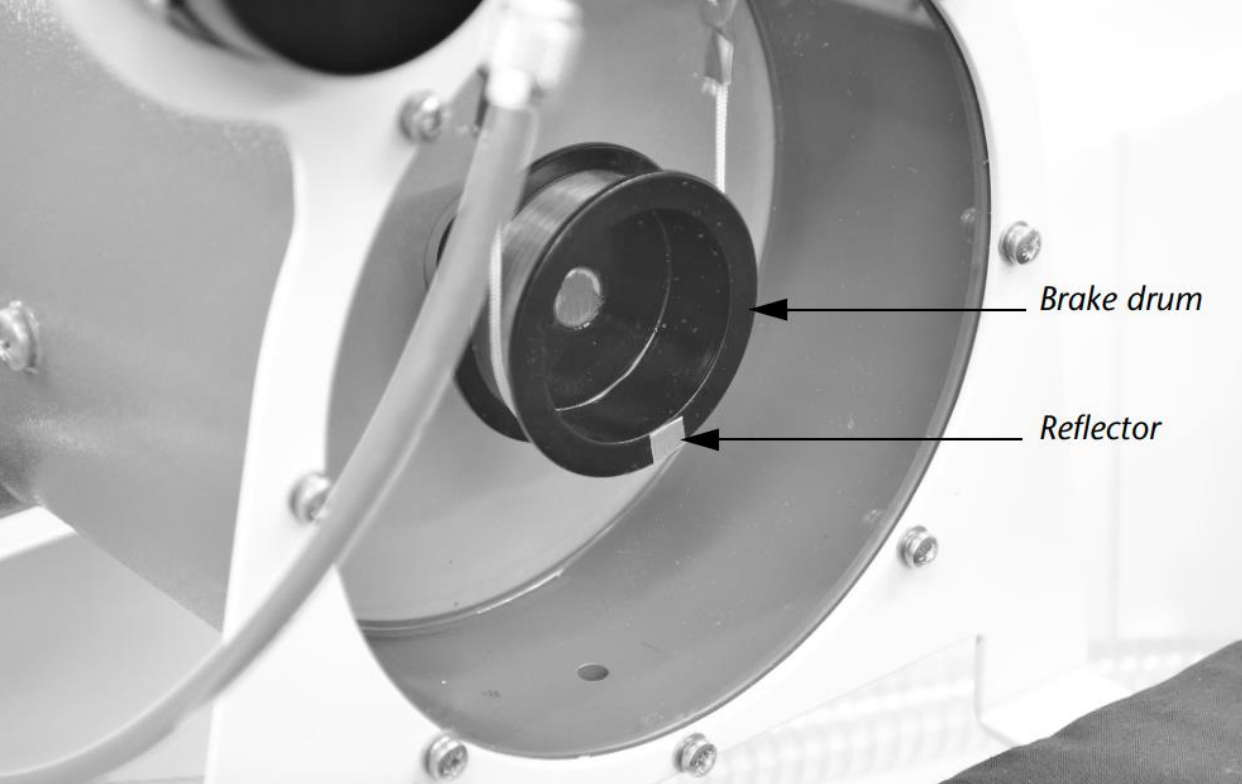
\includegraphics[width=0.55\textwidth]{Lab4_Figures/brake_drum_back.png}
    \caption{Back view of the turbine showing the brake drum and reflector region.}
    \label{fig:brake-drum}
\end{figure}

\section{Theoretical Background}

\subsection{Impulse Turbines}
An impulse turbine converts the kinetic energy of a high-speed water jet into rotational mechanical energy. Unlike a reaction turbine, an impulse turbine extracts energy primarily from a change in the momentum of the free jet as it passes over the moving blades.

The water jet exits the nozzle at high speed and strikes the blades mounted around the runner. The runner turns because the fluid leaves the blade with a different tangential momentum than it had at entry.

In this lab, the two blade shapes are intentionally different so students can investigate how turning the jet more strongly affects the torque and efficiency of the turbine.

\begin{figure}[H]
    \centering
    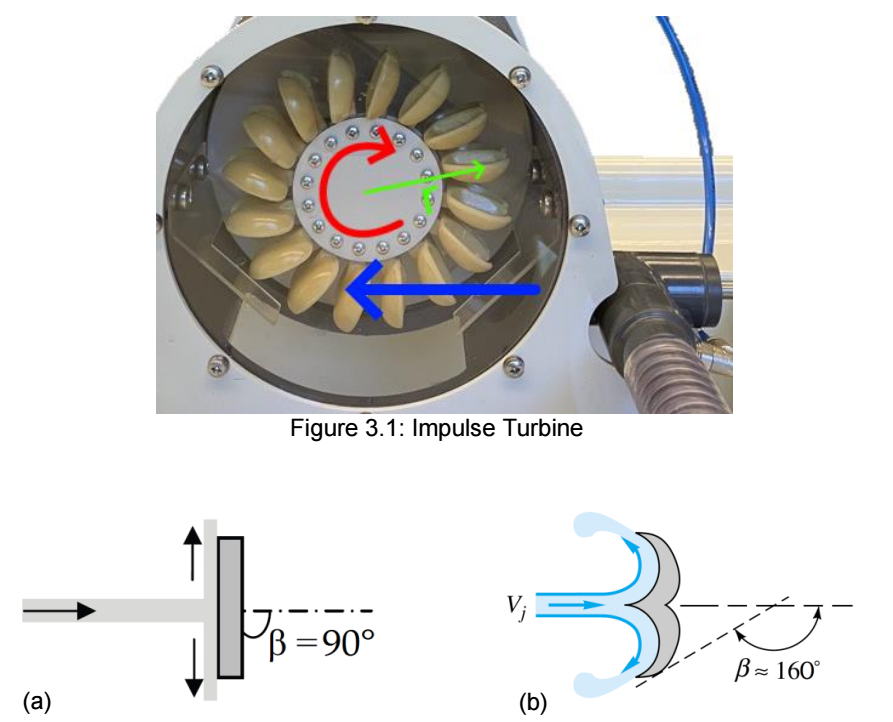
\includegraphics[width=0.62\textwidth]{Lab4_Figures/impulse_turbine_concept.png}
    \caption{Conceptual view of an impulse turbine with incoming jet, rotating runner, and shaft rotation.}
    \label{fig:impulse-concept}
\end{figure}

\subsection{Experimental Efficiency}
The measured or experimental efficiency of the turbine is defined as
\begin{equation}
\eta = \frac{\text{useful mechanical power output}}{\text{water-jet power input}}
= \frac{BHP}{P_w}
\label{eq:etaexpdef}
\end{equation}
where:
\begin{itemize}[leftmargin=*]
    \item \(BHP\) is the brake power delivered by the shaft,
    \item \(P_w\) is the kinetic power carried by the water jet.
\end{itemize}

\subsubsection*{Brake Power}
The brake power is
\begin{equation}
BHP = \omega T
\label{eq:bhp}
\end{equation}
where:
\begin{itemize}[leftmargin=*]
    \item \(\omega\) is the angular velocity in \(\text{rad/s}\),
    \item \(T\) is the shaft torque in \(\text{N}\cdot\text{m}\).
\end{itemize}

\subsubsection*{Water-Jet Power}
The kinetic power of the jet is
\begin{equation}
P_w = \frac{1}{2}\rho V_j^2 Q
\label{eq:pw}
\end{equation}
where:
\begin{itemize}[leftmargin=*]
    \item \(\rho\) is the density of water,
    \item \(V_j\) is the jet velocity,
    \item \(Q\) is the volumetric flow rate.
\end{itemize}

Combining Eq.~\eqref{eq:bhp} and Eq.~\eqref{eq:pw}, the experimental efficiency becomes
\begin{equation}
\eta = \frac{2\omega T}{\rho V_j^2 Q}.
\label{eq:etaexp}
\end{equation}

\subsection{Jet Velocity from the Pressure Gauge}
The jet velocity is estimated from the inlet pressure gauge using an energy-based relation:
\begin{equation}
V_j = C_v \sqrt{\frac{2P}{\rho}}
\label{eq:vj}
\end{equation}
where:
\begin{itemize}[leftmargin=*]
    \item \(P\) is the gauge pressure before the nozzle,
    \item \(C_v\) is a nozzle velocity coefficient used to account for losses.
\end{itemize}

For this lab,
\[
C_v = 0.95.
\]

Students should ensure that the pressure \(P\) is converted into SI units before using Eq.~\eqref{eq:vj}.

\subsection{Torque Measurement}
The shaft torque is measured indirectly using the brake drum and two load gauges. Because the right gauge reads higher than the left during rotation, the net brake force is
\begin{equation}
F_d = B - A
\label{eq:fd}
\end{equation}
where:
\begin{itemize}[leftmargin=*]
    \item \(A\) is the left gauge reading,
    \item \(B\) is the right gauge reading.
\end{itemize}

The torque is then
\begin{equation}
T = R_d F_d
\label{eq:torque}
\end{equation}
with
\[
R_d = 0.025~\text{m}.
\]

\begin{figure}[H]
    \centering
    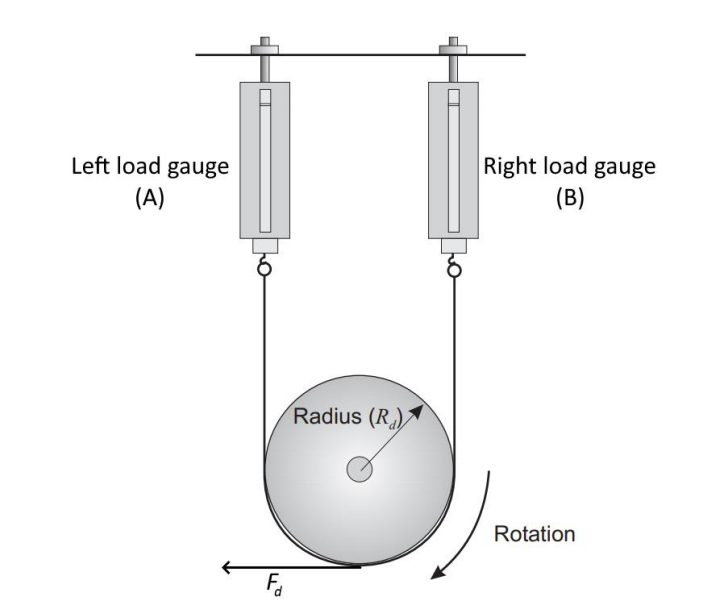
\includegraphics[width=0.52\textwidth]{Lab4_Figures/torque_measurements.png}
    \caption{Torque measurement using the two brake-load gauges and the brake drum radius.}
    \label{fig:torque-measurement}
\end{figure}

\subsection{Angular Velocity Measurement}
The turbine speed is measured in two ways:
\begin{enumerate}[leftmargin=*, label=\arabic*.]
    \item using a \textbf{stroboscope},
    \item using a \textbf{contactless optical tachometer}.
\end{enumerate}

For use in Eq.~\eqref{eq:bhp}, the angular speed must be in \(\text{rad/s}\). If the speed is measured in rpm, convert using
\begin{equation}
\omega = \frac{2\pi N}{60}
\label{eq:rpmtorads}
\end{equation}
where \(N\) is the rotational speed in revolutions per minute.

\subsection{Theoretical Efficiency from Angular Momentum}
The theoretical analysis is based on conservation of angular momentum. For steady flow, the shaft torque can be related to the inlet and outlet tangential momentum fluxes:
\begin{equation}
T_{\text{shaft}} = \dot{m}r_b\left(V_{\theta,\text{in}} - V_{\theta,\text{out}}\right)
\label{eq:tangmom}
\end{equation}
or, since \(\dot{m}=\rho Q\),
\begin{equation}
T_{\text{shaft}} = \rho Q r_b\left(V_{\theta,\text{in}} - V_{\theta,\text{out}}\right).
\label{eq:tangmom2}
\end{equation}

\begin{figure}[H]
    \centering
    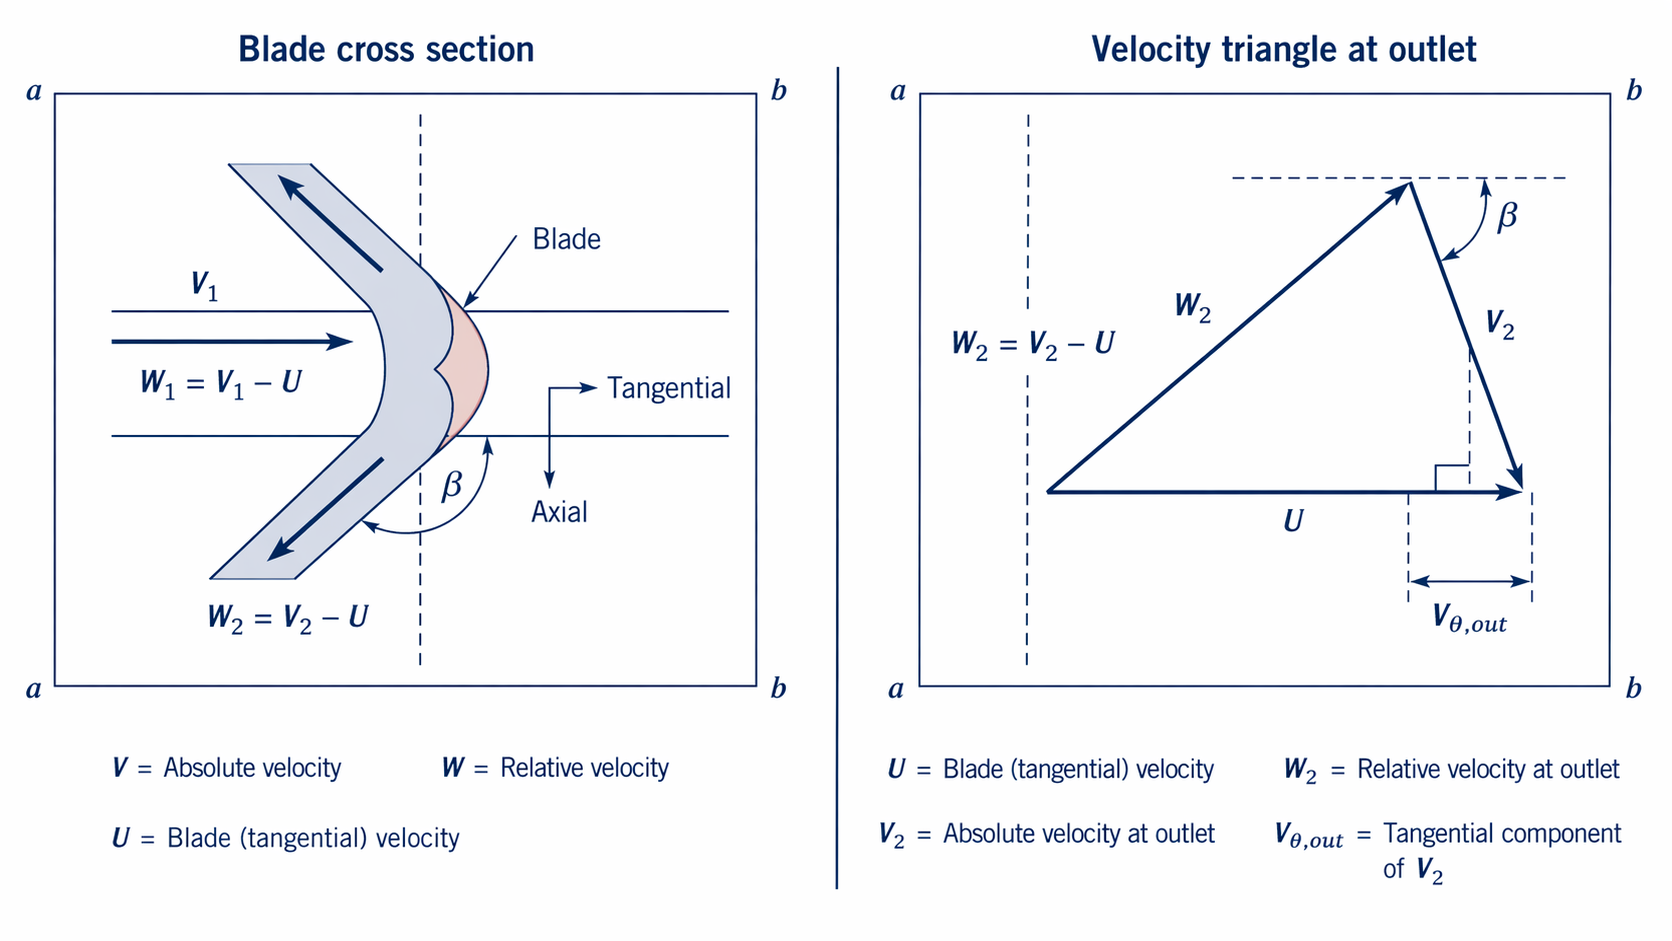
\includegraphics[width=0.78\textwidth]{Lab4_Figures/velocity_triangle.png}
    \caption{Velocity diagrams at turbine inlet and outlet used in the angular-momentum analysis.}
    \label{fig:velocity-diagrams}
\end{figure}

Figure~\ref{fig:velocity-diagrams} shows the inlet and outlet velocity triangles used to simplify the angular-momentum model. The incoming jet enters with tangential speed \(V_{\theta,\mathrm{in}}=V_j\), while the blade moves with peripheral speed \(V_b=r_b\omega\). Assuming negligible viscous loss along the blade surface, the relative speed is taken to be unchanged, so \(W_{\mathrm{in}}=W_{\mathrm{out}}\). The blade angle \(\beta\) then determines the outlet tangential component \(V_{\theta,\mathrm{out}}\), which directly controls the shaft torque.

Using the velocity-triangle relations for the blade and neglecting viscous losses inside the blade passage, the theoretical shaft torque becomes
\begin{equation}
T_{\text{shaft}} = \rho Q r_b \left(V_j - V_b\right)\left(1-\cos\beta\right)
\label{eq:torquetheory}
\end{equation}
where:
\begin{itemize}[leftmargin=*]
    \item \(r_b=0.046~\text{m}\) is the effective turbine radius (not the brake-drum radius),
    \item \(V_b\) is the peripheral blade speed,
    \item \(\beta\) is the blade turning angle.
\end{itemize}

The blade speed is
\begin{equation}
V_b = r_b\omega.
\label{eq:vb}
\end{equation}

Define the \textbf{peripheral velocity factor}
\begin{equation}
\phi = \frac{V_b}{V_j}.
\label{eq:phi}
\end{equation}

After substituting into the power relation and dividing by the jet power, the theoretical efficiency becomes
\begin{equation}
\eta_{\text{th}} = 2\phi(1-\phi)(1-\cos\beta).
\label{eq:etath}
\end{equation}

This is one of the key equations in the lab.

\subsection{Interpreting the Theoretical Efficiency Formula}
Equation~\eqref{eq:etath} shows several important ideas:
\begin{itemize}[leftmargin=*]
    \item The theoretical efficiency depends strongly on \(\beta\), the blade geometry.
    \item The efficiency is zero when \(\phi=0\) or \(\phi=1\).
    \item The efficiency is maximized at an intermediate value of blade speed relative to jet speed.
\end{itemize}

For the two turbines used here:
\begin{itemize}[leftmargin=*]
    \item \(\beta = 90^\circ\) for the flat blade,
    \item \(\beta = 160^\circ\) for the bucket (Pelton-type) blade.
\end{itemize}

Because the bucket blade turns the jet much more strongly, theory predicts that it should extract more angular momentum from the water and therefore achieve a higher efficiency.

\subsection{Useful student workflow for each data point}
For each operating point, students should calculate:
\begin{enumerate}[leftmargin=*, label=\arabic*.]
    \item \(F_d = B-A\),
    \item \(T = R_dF_d\), with \(R_d=0.025~\text{m}\),
    \item \(\omega = 2\pi N/60\),
    \item \(V_j = C_v\sqrt{2P/\rho}\),
    \item \(P_w = \frac{1}{2}\rho V_j^2Q\),
    \item \(BHP = \omega T\),
    \item \(\eta = BHP/P_w\),
    \item \(V_b = r_b\omega\), with \(r_b=0.046~\text{m}\),
    \item \(\phi = V_b/V_j\),
    \item \(\eta_{\text{th}} = 2\phi(1-\phi)(1-\cos\beta)\).
\end{enumerate}

\subsection{Stroboscope Notes for Students}
A stroboscope can make the rotating runner appear stationary when the flash frequency matches the rotation rate. If the strobe frequency is an integer multiple of the true rotation frequency, multiple apparent blade images may appear. Therefore, students should:
\begin{itemize}[leftmargin=*]
    \item use a distinctive feature on the runner or reflector as a reference,
    \item adjust the flash rate carefully,
    \item confirm the reading using the optical tachometer.
\end{itemize}

\section{Procedure}

\subsection*{Step-by-step procedure}
\begin{enumerate}[leftmargin=*, label=\arabic*.]
    \item Adjust the load until both gauges show no load. Do \textbf{not} zero the gauges.
    \item Fully open the spear valve until it is lightly seated. Do not use excessive force.
    \item Start the hydraulic bench and slowly open the flow valve until the flow rate is approximately \(10.5~\text{L/min}\).
    \item Measure the angular velocity of the turbine using the stroboscope and also using the contactless tachometer. Point the tachometer at the reflector. Record at least three angular velocities by adjusting the turbine brake load.
    \item Adjust the load until both gauges again show no load. Record the unloaded operation point in the main data table.
    \item Slowly increase the brake load in steps of \(0.5~\text{N}\). Record the angular velocity and load at each step.
    \item Continue until the turbine stops rotating. Turn the turbine manually to ensure the stopping-force value is maximized.
    \item When the first turbine is complete, reduce the load until both gauges show no load, close the flow valve fully, and turn off the hydraulic bench.
    \item Replace the first turbine with the second turbine of different blade geometry.
    \item Repeat the experiment for the second turbine. Step 4 need not be repeated if only one speed-comparison set is required.
\end{enumerate}

\subsection*{Recommended measurement practice for students}
\begin{itemize}[leftmargin=*]
    \item Record the pressure and flow rate at the same time as the speed and load readings.
    \item Increase the brake load gradually so the runner reaches steady rotation before recording data.
    \item Use consistent units throughout the analysis.
    \item Keep the pressure and flow settings as consistent as possible between the two turbine geometries.
    \item Near stall or very low speed, verify the speed carefully because rpm readings may fluctuate.
\end{itemize}

\begin{table}[H]
\centering
\caption{Angular velocity measurements using stroboscope and tachometer}
\label{tab:strobe-tach}
\begin{tabular}{cccc}
\toprule
Trial Number & Load Force (N) & Stroboscope [rpm] & Tachometer [rpm] \\
\midrule
1 & & & \\
2 & & & \\
3 & & & \\
\bottomrule
\end{tabular}
\end{table}

The unloaded point has \(F=0\) but should have the \emph{highest} nonzero rotational speed. Do not enter \(\omega=0\) for the unloaded point. Record the pressure and flow rate with each operating point so the companion notebook can calculate the jet velocity and water power from the actual conditions rather than a single nominal value.

\begin{table}[H]
\centering
\caption{Measurements for the flat-blade turbine, \(\beta=90^\circ\)}
\label{tab:main-data-90}
\begin{tabular}{ccccc}
\toprule
Trial & Net Brake Force \(F\) [N] & \(\omega\) [rpm] & \(P_g\) [kPa] & \(Q\) [L/min] \\
\midrule
1 & 0 & & & \\
2 & & & & \\
3 & & & & \\
4 & & & & \\
5 & & & & \\
6 & & & & \\
7 & & & & \\
8 & & & & \\
9 & & & & \\
10 & & & & \\
11 & & & & \\
12 & & & & \\
13 & & & & \\
14 & & & & \\
15 & & & & \\
\bottomrule
\end{tabular}
\end{table}

\begin{table}[H]
\centering
\caption{Measurements for the Pelton-type turbine, \(\beta=160^\circ\)}
\label{tab:main-data-160}
\begin{tabular}{ccccc}
\toprule
Trial & Net Brake Force \(F\) [N] & \(\omega\) [rpm] & \(P_g\) [kPa] & \(Q\) [L/min] \\
\midrule
1 & 0 & & & \\
2 & & & & \\
3 & & & & \\
4 & & & & \\
5 & & & & \\
6 & & & & \\
7 & & & & \\
8 & & & & \\
9 & & & & \\
10 & & & & \\
11 & & & & \\
12 & & & & \\
13 & & & & \\
14 & & & & \\
15 & & & & \\
\bottomrule
\end{tabular}
\end{table}

\section{Questions for Analysis}

\subsection*{Required calculations}
\begin{enumerate}[leftmargin=*, label=\arabic*.]
    \item For the \(\beta = 90^\circ\) and \(\beta = 160^\circ\) turbines, calculate the theoretical efficiency and plot it as a function of \(\phi\) ranging from 0 to 1.
    \item On the same plot, show the measured efficiency \(\eta\) for the \(\beta = 90^\circ\) and \(\beta = 160^\circ\) turbines.
    \item Determine the value of \(\phi\) at which the maximum efficiency is achieved. State whether the theoretical prediction matches the experimental observations.
    \item Explain the effect of \(\beta\) on the turbine efficiency, both theoretically and experimentally.
    \item Compare the stroboscopic and optical tachometer angular velocities.
\end{enumerate}

\subsection*{Suggested report structure for students}
Students are encouraged to structure the analysis section as follows:
\begin{enumerate}[leftmargin=*, label=\arabic*.]
    \item \textbf{Raw measurements:} present the recorded speed and load data.
    \item \textbf{Sample calculation:} show one complete worked example from raw data to efficiency. Explicitly distinguish the brake-drum radius \(R_d=0.025~\text{m}\), used in \(T=R_dF_d\), from the effective turbine radius \(r_b=0.046~\text{m}\), used in \(V_b=r_b\omega\) and \(\phi\).
    \item \textbf{Efficiency calculations:} tabulate \(\eta\), \(\phi\), and \(\eta_{\text{th}}\) for both turbines. Use the pressure and flow rate recorded for each operating point when evaluating \(V_j\) and \(P_w\).
    \item \textbf{Plots:} plot measured and theoretical efficiency on the same graph.
    \item \textbf{Discussion:} compare flat and bucket blade performance and explain the sources of discrepancy between theory and experiment.
\end{enumerate}

\subsection*{Discussion prompts}
Students should consider the following in the discussion:
\begin{itemize}[leftmargin=*]
    \item Why does the bucket-shaped blade perform better than the flat blade?
    \item Why do measured efficiencies usually lie below theoretical efficiencies?
    \item What losses are neglected in the theoretical model?
    \item Why does efficiency drop when the blade speed is either too small or too large relative to the jet speed?
    \item How reliable was the stroboscope compared with the tachometer?
\end{itemize}

\section*{References}
If external references are used in the discussion or supporting theory, include them in a proper references section at the end of the final report.

\section{Recommended Text Readings}

To fully prepare for the experimental and computational components of these labs, students are strongly encouraged to review the relevant sections in the course textbook. The following readings provide the theoretical foundation for the phenomena observed in the laboratory.

\vspace{0.3cm}
\noindent\textbf{Course Textbook Reference:} \\
White, F. M., \& Xue, H. (2020). \textit{Fluid Mechanics} (9th ed.). McGraw-Hill Education. \\
\textit{(*Note: Chapter and section numbering remains consistent with the 8th edition.)}
\vspace{0.3cm}



\subsection*{Lab 4: Turbomachinery -- Impulse Turbines}
\textbf{Primary Focus:} Angular momentum theorem, power extraction, and turbine efficiency.
\begin{itemize}
    \item \textbf{Chapter 3: Integral Relations for a Control Volume}
    \begin{itemize}
        \item Section 3.6: The Angular-Momentum Theorem
    \end{itemize}
    \item \textbf{Chapter 11: Turbomachinery}
    \begin{itemize}
        \item Section 11.1: Introduction and Classification
        \item Section 11.2: The Centrifugal Pump (Euler turbomachine equation)
        \item Section 11.5: Impulse Turbines (Pelton wheels, optimal bucket speed, and theoretical efficiency $\eta_{th}$)
    \end{itemize}
\end{itemize}
\begin{itemize}
        \item Dixon, S. L., \& Hall, C. A. (2013). \textit{Fluid Mechanics and Thermodynamics of Turbomachinery}. Butterworth-Heinemann. \url{https://doi.org/10.1016/C2011-0-05059-7}  \textit{(A deeper dive into velocity triangles, blade design, and efficiency matching).}
        \item Munson, B. R., et al. (2012). \textit{Fundamentals of Fluid Mechanics}. Wiley. \textit{(Contains highly practical diagrams on Pelton wheel momentum transfer).}
        \item TecQuipment Ltd. (2015). \textit{H19 Pelton Turbine User Guide}. \url{https://www.tecquipment.com/pelton-turbine} Technical details list a brake-drum radius of 25~mm and an effective turbine radius of 46~mm. Videos are available at the site. \textit{The link is for a newer version of the turbine}
    \end{itemize}

\end{document}
